%----------------------------------------------------------------------------------------
% EXPONENTIËLE EN MACHTSVERBANDEN. Alle opgaven zijn eigen werk. De gegevens zijn verzonnen, behalve de banen
% van de planeten (afgeronde waarden, zoals in elk naslagwerk) en waar een opgave een andere bron noemt.
%
% Opbouw: Probleem, Start, leerstof (theorie, werkwijze of uitleg, voorbeeld, korte oefening), en op een
% nieuwe pagina de Opdrachten (door elkaar, stijgende moeilijkheid), Koppel en Test jezelf.
% Labels van dit hoofdstuk beginnen met h3-.
%----------------------------------------------------------------------------------------

\mychapter{3}{Exponentiële en machtsverbanden}

\begin{probleem}
\naast{Johannes Kepler zocht jarenlang naar een verband tussen de afstand van een planeet tot de zon en de tijd die ze nodig heeft voor één omloop. In 1619 vond hij het. De tabel geeft voor de zes planeten die hij kende de gemiddelde afstand $a$ tot de zon (in astronomische eenheden, AE: de afstand van de aarde tot de zon) en de omlooptijd $T$ (in jaar).

\smallskip
{\small\setlength{\tabcolsep}{3.5pt}\renewcommand{\arraystretch}{1.25}\begin{tabular}{|>{\columncolor{accent!12}}l|c|c|c|c|c|c|}\hline
 & Mercurius & Venus & Aarde & Mars & Jupiter & Saturnus \\\hline
$a$ (AE) & 0,387 & 0,723 & 1 & 1,524 & 5,203 & 9,537 \\\hline
$T$ (jaar) & 0,241 & 0,615 & 1 & 1,881 & 11,86 & 29,46 \\\hline
\end{tabular}}

\smallskip
De punten liggen op een kromme, niet op een rechte. Welk verband is er? Kan lineaire regressie het vinden?}{\begin{tikzpicture}[x=.36cm,y=.105cm,font=\scriptsize]
  \diagram[$a$][$T$]{0}{2}{10}{0}{5}{30}
  \xas{0,2,...,10}\yas{0,10,20,30}
  \punten[inkt]{(0.387,0.241) (0.723,0.615) (1,1) (1.524,1.881) (5.203,11.86) (9.537,29.46)}
\end{tikzpicture}}
\end{probleem}

\lkr{Leerplan Complementair (III-WiCo-d): LPD 51 (het enkelvoudig lineair regressiemodel toepassen), met de wenk: machtsverbanden en exponentiële verbanden onderzoeken met lineaire regressie, door ze eerst met logaritmen lineair te maken, en de link met enkel- en dubbellogaritmisch papier. Het logaritmische model $y = A\ln x + B$ en de opmerking dat de kleinste kwadraten na de transformatie relatieve fouten meten, zijn extra. Voorkennis uit pakket 4: Exponentiële en logaritmische functies (exponentiële groei en verval met groeifactor, rekenregels van logaritmen, logaritmische schalen) en hoofdstuk 1 en 2 van dit boek. Op de TI-84: \texttt{ExpReg} geeft $y = a \cdot b^x$ en \texttt{PwrReg} geeft $y = a \cdot x^b$ (de letters van het toestel zijn niet die van dit boek); beide rekenen intern met de logaritmen, zoals in dit hoofdstuk. De gegevens van de planeten zijn afgeronde, algemeen bekende waarden; laat ze eventueel in een naslagwerk opzoeken.}

In hoofdstuk 2 zag je dat een hoge $R^2$ niet volstaat: soms toont de residuplot een boog, en dan is een rechte het verkeerde model. Maar de kleinste-kwadratenmethode werkt alleen voor modellen die lineair zijn in hun parameters. Wat dan met groei die telkens met dezelfde factor vermenigvuldigt, of met een wet zoals de remweg die met het kwadraat van de snelheid groeit? De oplossing is een oude truc: neem de logaritme. Een exponentieel verband en een machtsverband worden zo een lineair verband, en daarop werkt alles uit hoofdstuk 1 en 2. Op papier doe je hetzelfde met een logaritmische as. Op het einde vind je de wet van Kepler terug, zonder tien jaar te rekenen.

\begin{oefeningen}[Start]
\oef{h3-start-1}

\needspace{12\baselineskip}
\oef{h3-verken}
\end{oefeningen}

%========================================================================================
\section{Exponentiële verbanden}

\subsection{Lineair maken met een logaritme}

In hoofdstuk 2 telde een bioloog bacteriën in een kweek: 100, 150, 230, 340, 510 en 760 (duizend per ml) na 0 tot 5 uur. De residuplot toonde een boog. Elk uur vermenigvuldigt het aantal ongeveer met $1{,}5$: dat is exponentiële groei, $y = c \cdot g^x$ met beginwaarde $c$ en groeifactor $g$. Hoe vind je $c$ en $g$ met de kleinste kwadraten? Neem van beide leden de natuurlijke logaritme:
\[ \ln y = \ln c + x \ln g . \]
Dat is een rechte, met $x$ als veranderlijke en $\ln y$ als functiewaarde: helling $\ln g$, snijpunt $\ln c$.

\begin{theorie}
\begin{stelling}{Exponentieel verband}
Neem $c > 0$ en $g > 0$. De punten $(x_i, y_i)$ liggen op de kromme $\formule{y = c \cdot g^x}$ als en slechts als de punten $(x_i, \ln y_i)$ op de rechte $\formule{Y = Ax + B}$ liggen, met

\vspace{1mm}
\qquad $\formule{A = \ln g}$ \quad en \quad $\formule{B = \ln c}$, \quad dus \quad $\formule{g = \e^A}$ \quad en \quad $\formule{c = \e^B}$
\end{stelling}

\begin{bewijs}
Alle $y_i$ zijn positief, want $c \cdot g^x > 0$. Omdat $\ln$ een bijectie is van $\R^+_0$ naar $\R$, is
\bewijsregel{y_i = c \cdot g^{x_i} \iff \ln y_i = \ln c + x_i \ln g = B + A x_i .}
\end{bewijs}
\end{theorie}

Liggen de punten $(x_i, \ln y_i)$ niet precies op een rechte, dan zoek je de regressierechte van $\ln y$ op $x$, en vertaal je haar terug naar een exponentieel model. De groeifactor per eenheid $x$ is $g = \e^A$.

\voorbeeld{}{Bepaal een exponentieel model voor de bacteriën. Met welk percentage groeit de kweek per uur?\label{vb:h3-exp}}{%
\uitleg{We berekenen $\ln y$ voor elke meting, zoeken de regressierechte van $\ln y$ op $x$, en rekenen $A$ en $B$ terug naar $g$ en $c$.}
\begin{stappenbreed}
\ln y\colon\ 4{,}605;\ 5{,}011;\ 5{,}438;\ 5{,}829;\ 6{,}234;\ 6{,}633 & De logaritmen van de aantallen. \\[1ex]
Y \approx 0{,}4058x + 4{,}611 & \texttt{LinReg(ax+b)} met $x$ en $\ln y$; $r^2 \approx 0{,}9999$. \\[1ex]
g = \e^{0{,}4058} \approx 1{,}50, \quad c = \e^{4{,}611} \approx 100{,}5 & Terug naar het exponentiële model. \\[1ex]
y \approx 100{,}5 \cdot 1{,}50^x & Het model.
\end{stappenbreed}
\figuren{\begin{tikzpicture}[x=.6cm,y=.0042cm,font=\scriptsize]
  \diagram[$x$][$y$]{0}{1}{5}{0}{200}{800}
  \xas{0,1,...,5}\yas{0,200,...,800}
  \kromme{0}{5.2}{100.54*1.5005^\x}
  \punten[inkt]{(0,100) (1,150) (2,230) (3,340) (4,510) (5,760)}
\end{tikzpicture}\qquad
\begin{tikzpicture}[x=.6cm,y=1.3cm,font=\scriptsize]
  \diagram[$x$][$\ln y$]{0}{1}{5}{4}{0.5}{7}
  \xas{0,1,...,5}\yas{4,5,6,7}
  \rechte{0}{5.2}{0.4058}{4.6106}
  \punten[inkt]{(0,4.6052) (1,5.0106) (2,5.4381) (3,5.8289) (4,6.2344) (5,6.6333)}
\end{tikzpicture}}
Links de gegevens met het model, rechts de logaritmen met de regressierechte. Per uur vermenigvuldigt het aantal met $1{,}50$: een groei van 50~\% per uur. Met \texttt{ExpReg} geeft het rekentoestel meteen $y = a \cdot b^x$ met $a \approx 100{,}5$ en $b \approx 1{,}50$.}

\begin{werkwijze}
Controleer dat alle $y_i > 0$. Bereken $Y_i = \ln y_i$ en de regressierechte $Y = Ax + B$ van $\ln y$ op $x$. Het model is $y = c \cdot g^x$ met $g = \e^A$ en $c = \e^B$. Kijk naar de residuplot van $(x_i, \ln y_i)$ om te zien of het model past. Of: \texttt{ExpReg}, met $a = c$ en $b = g$.
\end{werkwijze}

\begin{oefeningen}
\oef{h3-exp}
\end{oefeningen}

\subsection{Verval en halveringstijd}

Bij verval is de groeifactor kleiner dan 1, en de helling $A = \ln g$ negatief. Wat vaak gevraagd wordt, is de halveringstijd: de tijd waarin de grootheid halveert. Uit $g^h = \frac12$ volgt $h = \frac{\ln 0{,}5}{\ln g} = \frac{-\ln 2}{A}$.

\voorbeeld{}{Na een inspuiting meet een arts om de twee uur de concentratie $C$ van een geneesmiddel in het bloed (in mg/l).

\smallskip
\kleinetabel[$t$ (uur)][$C$ (mg/l)]{6}{0 & 2 & 4 & 6 & 8 & 10}{12{,}0 & 8{,}6 & 6{,}1 & 4{,}4 & 3{,}1 & 2{,}2}

\smallskip
Bepaal een exponentieel model en de halveringstijd.\label{vb:h3-verval}}{%
\uitleg{Elke twee uur daalt de concentratie met ongeveer dezelfde factor ($\frac{8{,}6}{12} \approx 0{,}72$, $\frac{6{,}1}{8{,}6} \approx 0{,}71$): verval. We regresseren $\ln C$ op $t$.}
\begin{stappenbreed}
Y \approx -0{,}1696t + 2{,}489 & Regressierechte van $\ln C$ op $t$. \\[1ex]
g = \e^{-0{,}1696} \approx 0{,}844, \quad c = \e^{2{,}489} \approx 12{,}05 & Per uur blijft 84,4~\% over. \\[1ex]
h = \frac{-\ln 2}{-0{,}1696} \approx 4{,}1 & De halveringstijd in uur.
\end{stappenbreed}
Het model is $C \approx 12{,}05 \cdot 0{,}844^t$: per uur verdwijnt ongeveer 15,6~\% van het geneesmiddel, en na ongeveer 4,1 uur is de concentratie gehalveerd.}

\begin{oefeningen}
\oef{h3-verval}
\end{oefeningen}

%========================================================================================
\section{Enkellogaritmisch papier}

Vóór er rekentoestellen waren, tekende men $\ln y$ niet zelf: men gebruikte papier waarop de $y$-as al logaritmisch verdeeld is. Op zo'n as staat $y$ op de hoogte $\log y$. De afstand van 1 tot 10 is dezelfde als van 10 tot 100, en tussen twee machten van 10 liggen de lijnen voor $2, 3, \ldots, 9$ steeds dichter bij elkaar.

\begin{theorie}
Op \textbf{\textcolor{accent}{enkellogaritmisch papier}} is de $x$-as gewoon verdeeld en de $y$-as logaritmisch: een punt $(x, y)$ staat op de hoogte $\log y$.

\begin{stelling}{Rechte op enkellogaritmisch papier}
Een exponentieel verband $\formule{y = c \cdot g^x}$ is op enkellogaritmisch papier een rechte. Bij elke stap van 1 in $x$ stijgt de rechte met $\formule{\log g}$.
\end{stelling}

\begin{bewijs}
De hoogte van het punt is $\log y = \log c + x\log g$: een eerstegraadsfunctie van $x$, met helling $\log g$.
\end{bewijs}
\end{theorie}

Het maakt niet uit of je $\ln$ of $\log$ gebruikt: $\ln y = \ln 10 \cdot \log y$, dus beide rechten verschillen alleen in schaal. Het papier gebruikt $\log$, het rekentoestel $\ln$.

\naast{\begin{minipage}{9.4cm}
Rechts staan de bacteriën op enkellogaritmisch papier, met de regressierechte uit voorbeeld \ref{vb:h3-exp}. De punten liggen op een rechte. Je leest er ook de verdubbelingstijd af: van 100 tot 200 is even ver als van 200 tot 400. De rechte stijgt van 100 naar 200 in ongeveer $1{,}7$ uur, want $1{,}5^{1{,}7} \approx 2$.

\smallskip
Waarom is zo'n papier handig? Je ziet meteen of groei exponentieel is (een rechte), of de groeifactor verandert (een knik), en grootheden die over vele machten van 10 lopen, passen op één blad.
\end{minipage}}{\begin{tikzpicture}[x=.75cm,y=3cm,font=\scriptsize]
  \logy{0}{5}{2}{3}
  \foreach \t in {1,...,5}{\draw[black!12,very thin] (\t,2) -- (\t,3);}
  \draw[->,grijs] (0,2) -- (5.4,2) node[right,text=black] {$x$};
  \draw[->,grijs] (0,2) -- (0,3.12) node[above,text=black] {$y$};
  \foreach \t in {0,...,5}{\node[below] at (\t,2) {$\t$};}
  \foreach \v in {100,200,300,500,1000}{\node[left] at (0,{log10(\v)}) {$\v$};}
  \draw[accent,thick] (0,{log10(100.54)}) -- (5.2,{log10(100.54)+5.2*log10(1.5005)});
  \punten[inkt]{(0,2) (1,2.1761) (2,2.3617) (3,2.5315) (4,2.7076) (5,2.8808)}
  \draw[fel!80!black,thick,densely dashed] (0,2.301) -- (1.71,2.301) -- (1.71,2);
\end{tikzpicture}}

\voorbeeld{}{Op enkellogaritmisch papier gaat een rechte door de punten $(0, 50)$ en $(4, 800)$. Bepaal het exponentiële verband.\label{vb:h3-papier}}{%
\uitleg{Een rechte op dit papier is een exponentieel verband $y = c \cdot g^x$. De waarde bij $x = 0$ geeft $c$, en de verhouding van de $y$-waarden geeft $g$.}
\begin{stappenbreed}
c = 50 & De waarde bij $x = 0$. \\[1ex]
g^4 = \frac{800}{50} = 16, \quad\text{dus } g = 2 & In 4 stappen vermenigvuldigt $y$ met 16. \\[1ex]
y = 50 \cdot 2^x & Het verband.
\end{stappenbreed}
Je hoeft geen logaritmen te berekenen: op het papier staan de waarden van $y$ zelf.}

\begin{oefeningen}
\oef{h3-papier}
\end{oefeningen}

%========================================================================================
\section{Machtsverbanden}

\subsection{Lineair maken met twee logaritmen}

Niet elke kromme is exponentieel. De periode $T$ van een slinger groeit met de lengte $L$, maar niet met een vaste factor per meter: ze is evenredig met $\sqrt L$. Zo'n verband $y = c \cdot x^p$, met een vaste exponent $p$, heet een machtsverband. Neem weer de logaritme:
\[ \ln y = \ln c + p\ln x . \]
Nu is $\ln y$ een eerstegraadsfunctie van $\ln x$: je hebt beide logaritmen nodig.

\begin{theorie}
\begin{stelling}{Machtsverband}
Neem $c > 0$ en $x_i > 0$. De punten $(x_i, y_i)$ liggen op de kromme $\formule{y = c \cdot x^p}$ als en slechts als de punten $(\ln x_i, \ln y_i)$ op de rechte $\formule{Y = AX + B}$ liggen, met

\vspace{1mm}
\qquad $\formule{A = p}$ \quad en \quad $\formule{B = \ln c}$, \quad dus \quad $\formule{c = \e^B}$
\end{stelling}

\begin{bewijs}
Voor $x_i > 0$ is $y_i = c \cdot x_i^p > 0$, en
\bewijsregel{y_i = c \cdot x_i^p \iff \ln y_i = \ln c + p\ln x_i = B + A\ln x_i .}
\end{bewijs}
\end{theorie}

De helling is hier zelf de exponent, zonder terugrekenen. Ze heeft ook een betekenis: wordt $x$ twee keer zo groot, dan wordt $y$ $2^p$ keer zo groot, onafhankelijk van waar je begint.

\voorbeeld{}{Leerlingen meten de periode $T$ (in s) van een slinger bij zes lengtes $L$ (in m).

\smallskip
\kleinetabel[$L$ (m)][$T$ (s)]{6}{0{,}2 & 0{,}4 & 0{,}6 & 0{,}8 & 1{,}0 & 1{,}2}{0{,}90 & 1{,}27 & 1{,}55 & 1{,}79 & 2{,}01 & 2{,}19}

\smallskip
Bepaal een machtsverband. Volgens de fysica is $T \approx 2{,}006\,L^{0{,}5}$ (dat is $2\pi$ gedeeld door de wortel uit de valversnelling $9{,}81$~m/s$^2$). Kloppen de metingen?\label{vb:h3-macht}}{%
\uitleg{We berekenen $\ln L$ en $\ln T$, en zoeken de regressierechte van $\ln T$ op $\ln L$.}
\begin{stappenbreed}
\ln L\colon\ {-1{,}609};\ {-0{,}916};\ {-0{,}511};\ {-0{,}223};\ 0;\ 0{,}182 & De logaritmen van de lengtes. \\[1ex]
\ln T\colon\ {-0{,}105};\ 0{,}239;\ 0{,}438;\ 0{,}582;\ 0{,}698;\ 0{,}784 & De logaritmen van de periodes. \\[1ex]
Y \approx 0{,}4973X + 0{,}6944 & Regressierechte van $\ln T$ op $\ln L$. \\[1ex]
p \approx 0{,}497, \quad c = \e^{0{,}6944} \approx 2{,}003 & Terug naar het machtsverband.
\end{stappenbreed}
Het model $T \approx 2{,}003\,L^{0{,}497}$ ligt heel dicht bij de theorie. \texttt{PwrReg} geeft hetzelfde: $y = a \cdot x^b$ met $a \approx 2{,}003$ en $b \approx 0{,}497$.}

\begin{werkwijze}
Controleer dat alle $x_i > 0$ en $y_i > 0$. Bereken $X_i = \ln x_i$ en $Y_i = \ln y_i$, en de regressierechte $Y = AX + B$. Het model is $y = c \cdot x^p$ met $p = A$ en $c = \e^B$. Of: \texttt{PwrReg}, met $a = c$ en $b = p$.
\end{werkwijze}

\begin{oefeningen}
\oef{h3-macht}
\end{oefeningen}

\subsection{Dubbellogaritmisch papier}

Op \textbf{dubbellogaritmisch papier} zijn beide assen logaritmisch. Een machtsverband $y = c \cdot x^p$ is daarop een rechte, want $\log y = \log c + p\log x$. De helling meet je in decaden: stijgt de rechte twee decaden terwijl ze één decade naar rechts gaat, dan is $p = 2$. Bij $x = 1$ lees je $c$ af, want $1^p = 1$.

\naast{\begin{minipage}{9.4cm}
Rechts zie je de slinger op dubbellogaritmisch papier. Van $L = 0{,}2$ tot $L = 0{,}8$ wordt de lengte vier keer zo groot, en de periode ongeveer twee keer: $1{,}79 \approx 2 \cdot 0{,}90$. Dat is $4^{0{,}5} = 2$. Bij $L = 1$ lees je $c \approx 2$ af.

\smallskip
Op enkellogaritmisch papier zou de slinger geen rechte zijn, en een exponentieel verband is op dubbellogaritmisch papier geen rechte. Het soort papier waarop de punten een rechte vormen, zegt dus welk model past.
\end{minipage}}{\begin{tikzpicture}[x=4cm,y=4cm,font=\scriptsize]
  \begin{scope}
  \clip (-0.75,-0.1) rectangle (0.15,0.5);
  \logy{-1}{1}{-1}{1}
  \logx{-1}{1}{-1}{1}
  \end{scope}
  \draw[->,grijs] (-0.75,-0.1) -- (0.2,-0.1) node[right,text=black] {$L$};
  \draw[->,grijs] (-0.75,-0.1) -- (-0.75,0.56) node[above,text=black] {$T$};
  \foreach \v/\l in {0.2/{0,2},0.4/{0,4},0.6/{0,6},1/1}{\node[below] at ({log10(\v)},-0.1) {$\l$};}
  \foreach \v/\l in {1/1,2/2,3/3}{\node[left] at (-0.75,{log10(\v)}) {$\l$};}
  \draw[accent,thick] (-0.74,{0.30157+0.4973*(-0.74)}) -- (0.12,{0.30157+0.4973*0.12});
  \punten[inkt]{(-0.699,-0.0458) (-0.3979,0.1038) (-0.2218,0.1903) (-0.0969,0.2529) (0,0.3032) (0.0792,0.3404)}
\end{tikzpicture}}

\voorbeeld{}{Op dubbellogaritmisch papier gaat een rechte door de punten $(1, 5)$ en $(100, 0{,}05)$. Bepaal het machtsverband.\label{vb:h3-dubbel}}{%
\uitleg{Een rechte op dit papier is een machtsverband $y = c \cdot x^p$. Bij $x = 1$ lees je $c$ af; de helling in decaden geeft $p$.}
\begin{stappenbreed}
c = 5 & De waarde bij $x = 1$. \\[1ex]
p = \frac{\log 0{,}05 - \log 5}{\log 100 - \log 1} = \frac{-2}{2} = -1 & Twee decaden naar beneden over twee decaden naar rechts. \\[1ex]
y = 5x^{-1} = \frac{5}{x} & Het verband.
\end{stappenbreed}
Een machtsverband met een negatieve exponent is dalend: $y$ is omgekeerd evenredig met $x$.}

\begin{oefeningen}
\oef{h3-dubbel}
\end{oefeningen}

%========================================================================================
\section{Welk model?}

\subsection{De juiste transformatie kiezen}

Hoe weet je welk model past? Elk model heeft een eigen transformatie die het tot een rechte maakt. Teken de getransformeerde punten, en kijk welke het best op een rechte liggen: zonder boog in de residuplot. De tabel geeft de vier modellen die je met ICT kunt berekenen.

\figuren{\renewcommand{\arraystretch}{1.5}\begin{tabular}{|c|c|c|c|}\hline
\textbf{model} & \textbf{rechte tussen} & \textbf{papier} & \textbf{ICT} \\\hline
lineair $y = ax + b$ & $x$ en $y$ & gewoon & \texttt{LinReg(ax+b)} \\\hline
exponentieel $y = c \cdot g^x$ & $x$ en $\ln y$ & enkellogaritmisch ($y$) & \texttt{ExpReg} \\\hline
macht $y = c \cdot x^p$ & $\ln x$ en $\ln y$ & dubbellogaritmisch & \texttt{PwrReg} \\\hline
logaritmisch $y = A\ln x + B$ & $\ln x$ en $y$ & enkellogaritmisch ($x$) & \texttt{LnReg} \\\hline
\end{tabular}}

\voorbeeld{}{Kies tussen een exponentieel model en een machtsverband voor de punten $(1;\ 3{,}1)$, $(2;\ 10{,}2)$, $(3;\ 21{,}5)$, $(4;\ 36{,}0)$, $(5;\ 53{,}8)$ en $(6;\ 76{,}1)$.\label{vb:h3-kies}}{%
\uitleg{We tekenen $\ln y$ tegenover $x$ en tegenover $\ln x$, en vergelijken de residuen van beide regressierechten.}
\figuren{\begin{tikzpicture}[x=.6cm,y=.9cm,font=\scriptsize]
  \diagram[$x$][$\ln y$]{0}{1}{6}{0}{1}{5}
  \xas{0,2,4,6}\yas{0,1,...,5}
  \rechte{0.5}{6.3}{0.6145}{0.9197}
  \punten[inkt]{(1,1.1314) (2,2.3224) (3,3.0681) (4,3.5835) (5,3.9853) (6,4.332)}
\end{tikzpicture}\qquad
\begin{tikzpicture}[x=1.8cm,y=.9cm,font=\scriptsize]
  \diagram[$\ln x$][$\ln y$]{0}{0.5}{2}{0}{1}{5}
  \xas{0,1,2}\yas{0,1,...,5}
  \rechte{0}{1.95}{1.7868}{1.1111}
  \punten[inkt]{(0,1.1314) (0.6931,2.3224) (1.0986,3.0681) (1.3863,3.5835) (1.6094,3.9853) (1.7918,4.332)}
\end{tikzpicture}}
\begin{stappenbreed}
\text{exponentieel: } r^2 \approx 0{,}942 & Regressie van $\ln y$ op $x$. \\[1ex]
\text{residuen } {-0{,}40};\ 0{,}17;\ 0{,}30;\ 0{,}21;\ {-0{,}01};\ {-0{,}27} & Een duidelijke boog. \\[1ex]
\text{macht: } r^2 \approx 0{,}9998 & Regressie van $\ln y$ op $\ln x$. \\[1ex]
\text{residuen tussen } {-0{,}03} \text{ en } 0{,}02 & Geen patroon. \\[1ex]
y \approx \e^{1{,}111} x^{1{,}787} \approx 3{,}04\,x^{1{,}79} & Het machtsverband.
\end{stappenbreed}
Links buigen de punten af: de groei vertraagt, wat bij een exponentieel model niet kan. Rechts liggen ze op een rechte. Het machtsverband past.}

\begin{werkwijze}
Teken de punten (of laat ICT ze tekenen) in de transformaties van de tabel. Kies het model waarvan de getransformeerde punten op een rechte liggen, zonder boog in de residuplot. Vergelijk geen $r^2$ van modellen met een verschillende $y$-variabele ($y$ of $\ln y$) als enig criterium: ze meten iets anders. Denk ook na over de context: begint de grootheid bij 0 (een macht met $p > 0$) of bij een beginwaarde (exponentieel)?
\end{werkwijze}

\begin{oefeningen}
\oef{h3-kies}

\oef{h3-lnreg}
\end{oefeningen}

\subsection{Wat minimaliseert de transformatie?}

Na de transformatie maak je de residuen van $\ln y$ zo klein mogelijk, niet die van $y$. Is dat erg? Een residu $\ln y_i - \ln \yhat_i = \ln \frac{y_i}{\yhat_i}$ is voor kleine afwijkingen ongeveer de relatieve fout $\frac{y_i - \yhat_i}{\yhat_i}$. De methode behandelt dus een fout van 10~\% bij een groot aantal even zwaar als een fout van 10~\% bij een klein aantal. Bij groei over vele machten van 10 is dat net wat je wilt: met de kleinste kwadraten op $y$ zelf zouden de grootste waarden alles bepalen. Maar het model is niet de kromme met de kleinste kwadratensom in $y$; die vind je alleen met een numerieke methode.

\voorbeeld{}{Een model voorspelt $\yhat = 200$, en de meting is $y = 220$. Vergelijk het residu van $\ln y$ met de relatieve fout. Doe hetzelfde bij $\yhat = 2$ en $y = 2{,}2$.\label{vb:h3-relatief}}{%
\uitleg{We berekenen $\ln y - \ln \yhat = \ln \frac{y}{\yhat}$ en $\frac{y - \yhat}{\yhat}$.}
\begin{stappenbreed}
\ln \tfrac{220}{200} = \ln 1{,}1 \approx 0{,}0953, \qquad \tfrac{20}{200} = 0{,}1 & Bij het grote aantal. \\[1ex]
\ln \tfrac{2{,}2}{2} = \ln 1{,}1 \approx 0{,}0953, \qquad \tfrac{0{,}2}{2} = 0{,}1 & Bij het kleine aantal: hetzelfde.
\end{stappenbreed}
In $y$ verschillen de residuen een factor 100 (20 tegenover 0,2), en hun kwadraten een factor $10\,000$. In $\ln y$ zijn ze gelijk, en ongeveer gelijk aan de relatieve fout.}

\begin{oefeningen}
\oef{h3-relatief}
\end{oefeningen}

%========================================================================================
\needspace{16\baselineskip}
\subsection{Terug naar het probleem}

\voorbeeld{}{Terug naar het probleem. Johannes Kepler zocht jarenlang naar een verband tussen de gemiddelde afstand $a$ van een planeet tot de zon (in AE, de afstand van de aarde tot de zon) en haar omlooptijd $T$ (in jaar). Voor de zes planeten die hij kende, zijn de koppels $(a, T)$: Mercurius $(0{,}387;\ 0{,}241)$, Venus $(0{,}723;\ 0{,}615)$, Aarde $(1;\ 1)$, Mars $(1{,}524;\ 1{,}881)$, Jupiter $(5{,}203;\ 11{,}86)$ en Saturnus $(9{,}537;\ 29{,}46)$. De punten liggen op een kromme, niet op een rechte. Welk model past? Bepaal het met lineaire regressie, en vergelijk met de derde wet van Kepler: $T^2 = a^3$.\label{vb:h3-terug}}{%
\uitleg{De afstanden lopen van 0,4 tot 10 AE, de omlooptijden van 0,24 tot 30 jaar: logaritmen liggen voor de hand. We proberen een rechte, een exponentieel model en een machtsverband.}
\begin{stappenbreed}
\text{lineair: } r^2 \approx 0{,}985 & Regressie van $T$ op $a$. \\[1ex]
\text{residuen } 1{,}24;\ 0{,}54;\ 0{,}05;\ {-0{,}74};\ {-2{,}46};\ 1{,}36 & Een boog. \\[1ex]
\text{exponentieel: } r^2 \approx 0{,}883 & Slecht, met een boog. \\[1ex]
\ln a\colon\ {-0{,}949};\ {-0{,}324};\ 0;\ 0{,}421;\ 1{,}649;\ 2{,}255 & Voor het machtsverband. \\[1ex]
\ln T\colon\ {-1{,}423};\ {-0{,}486};\ 0;\ 0{,}632;\ 2{,}473;\ 3{,}383 & \\[1ex]
Y \approx 1{,}4997X + 0{,}0003, \quad r^2 \approx 1{,}0000 & Residuen kleiner dan $0{,}001$. \\[1ex]
T \approx 1{,}000 \cdot a^{1{,}500} & Het machtsverband.
\end{stappenbreed}
\naast{\begin{minipage}{8.8cm}
De punten $(\ln a, \ln T)$ liggen zo goed als perfect op een rechte met helling $1{,}5$ en snijpunt 0. Dus $T = a^{1{,}5}$, en in het kwadraat $T^2 = a^3$: de derde wet van Kepler. Dat het snijpunt 0 is, komt van de eenheden: de aarde heeft $a = 1$ en $T = 1$. Een lineair model gaf $r^2 \approx 0{,}985$, maar de residuplot verraadt dat het verkeerd is. Kepler vond de wet in 1618, na jaren van rekenen en proberen. Logaritmen waren toen nog nieuw: John Napier publiceerde ze in 1614. Isaac Newton verklaarde de wet later met zijn gravitatiewet.
\end{minipage}}{\begin{tikzpicture}[x=1.6cm,y=1.1cm,font=\scriptsize]
  \logy{-1}{1}{-1}{2}
  \logx{-1}{2}{-1}{1}
  \draw[->,grijs] (-1,-1) -- (1.2,-1) node[right,text=black] {$a$};
  \draw[->,grijs] (-1,-1) -- (-1,2.2) node[above,text=black] {$T$};
  \foreach \v/\l in {-1/{0,1},0/1,1/10}{\node[below] at (\v,-1) {$\l$};}
  \foreach \v/\l in {-1/{0,1},0/1,1/10,2/100}{\node[left] at (-1,\v) {$\l$};}
  \draw[accent,thick] (-0.6667,-1) -- (1,1.5);
  \punten[inkt]{(-0.4123,-0.618) (-0.1409,-0.2111) (0,0) (0.183,0.2744) (0.7162,1.0741) (0.9794,1.4692)}
\end{tikzpicture}}}

%========================================================================================
\opdrachtenkop

\begin{oefeningen}
\oef{h3-o1}

\needspace{10\baselineskip}
\oef{h3-o2}

\oef{h3-o3}

\needspace{10\baselineskip}
\oef{h3-o4}

\oef{h3-o5}

\needspace{12\baselineskip}
\oef{h3-o6}

\oef{h3-o7}

\needspace{12\baselineskip}
\oef{h3-o8}

\oef{h3-o9}

\needspace{12\baselineskip}
\oef{h3-o10}

\oef{h3-o11}

\needspace{12\baselineskip}
\oef{h3-o12}

\oef{h3-o13}

\needspace{12\baselineskip}
\oef{h3-o14}

\oef{h3-o15}

\needspace{12\baselineskip}
\oef{h3-o16}

\oef{h3-o17}

\needspace{12\baselineskip}
\oef{h3-o18}

\oef{h3-o19}

\needspace{12\baselineskip}
\oef{h3-o20}

\oef{h3-o21}

\needspace{12\baselineskip}
\oef{h3-o22}
\end{oefeningen}

%----------------------------------------------------------------------------------------
% KOPPEL: verbanden met andere leerstof
%----------------------------------------------------------------------------------------
\needspace{20\baselineskip}
\opdrachtsectie{Koppel}

\lkr{De eerste oefening steunt op Rijen (meetkundige rijen), de tweede op Limieten en afgeleiden (de afgeleide van een machtsfunctie, relatieve verandering), de derde op Exponentiële en logaritmische functies (logaritmische schalen: decibel en de wet van het kwadraat van de afstand).}

\begin{oefeningen}
\oef{h3-koppel-1}

\oef{h3-koppel-2}

\oef{h3-koppel-3}
\end{oefeningen}

%----------------------------------------------------------------------------------------
\opdrachtsectie{Test jezelf}

\begin{oefeningen}
\oef{h3-t1}

\oef{h3-t2}

\oef{h3-t3}

\oef{h3-t4}

\oef{h3-t5}

\oef{h3-t6}

\oef{h3-t7}
\end{oefeningen}

\herhaalschema{%
  \fv{oef:h3-t1}{vb:h3-exp}{oef:h3-exp}%
  \fv{oef:h3-t2}{vb:h3-verval}{oef:h3-verval}%
  \fv{oef:h3-t3}{vb:h3-papier}{oef:h3-papier}%
  \fv{oef:h3-t4}{vb:h3-macht}{oef:h3-macht}%
  \fv{oef:h3-t5}{vb:h3-dubbel}{oef:h3-dubbel}%
  \fv{oef:h3-t6}{vb:h3-kies}{oef:h3-kies}%
  \fv{oef:h3-t7}{vb:h3-exp}{oef:h3-o1}}

\ifzelfstudie
\section*{Maak je eigen samenvatting}
Sluit dit boek en schrijf in je schrift: hoe je een exponentieel verband en een machtsverband met logaritmen lineair maakt (met bewijs), hoe je $c$, $g$ en $p$ terugrekent, de halveringstijd, wat enkel- en dubbellogaritmisch papier is en waarom de verbanden daarop rechten zijn, hoe je $c$ en $p$ of $g$ van zo'n papier afleest, de tabel met de vier modellen, hoe je het juiste model kiest, en wat de transformatie met de residuen doet. Vergelijk daarna met de kaders.
\fi
